\documentclass[conference]{IEEEtran}


%\usepackage{geometry}
\usepackage{amsmath}
\usepackage{amssymb}
\usepackage{amsthm}
\usepackage{times}
\usepackage{helvet}
\usepackage{courier}
\usepackage{graphicx}
\usepackage{subfigure}
\usepackage{mdwmath}
\usepackage{mdwtab}
\usepackage{amssymb}
\usepackage{booktabs}
\usepackage{algorithm}
\usepackage{pifont}
\usepackage{algpseudocode}
\usepackage{balance}
\usepackage{bm}
\usepackage{ulem}
\usepackage{array}
\usepackage{balance}
\usepackage{multirow}
\usepackage{multicol}
\usepackage{threeparttable}
\frenchspacing
\usepackage[marginal]{footmisc}
\usepackage{extarrows}
\usepackage{natbib}

%add the command initial
\algnewcommand\algorithmicInitial{\textbf{Initialize:}}
\algnewcommand\Initial{\item[\algorithmicInitial]}
\algnewcommand\algorithmicIterate{\textbf{Iterate:}}
\algnewcommand\Iterate{\item[\algorithmicIterate]}



\ifCLASSINFOpdf

\else

\fi



% correct bad hyphenation here
\hyphenation{op-tical net-works semi-conduc-tor}


\begin{document}
%
% paper title
% Titles are generally capitalized except for words such as a, an, and, as,
% at, but, by, for, in, nor, of, on, or, the, to and up, which are usually
% not capitalized unless they are the first or last word of the title.
% Linebreaks \\ can be used within to get better formatting as desired.
% Do not put math or special symbols in the title.
%\title{Bare Demo of IEEEtran.cls\\ for IEEE Conferences}
\title{Speed Maintained SVRG}

% author names and affiliations
% use a multiple column layout for up to three different
% affiliations
\author{\IEEEauthorblockN{Michael Shell}
\IEEEauthorblockA{School of Electrical and\\Computer Engineering\\
Georgia Institute of Technology\\
Atlanta, Georgia 30332--0250\\
Email: http://www.michaelshell.org/contact.html}
\and
\IEEEauthorblockN{Homer Simpson}
\IEEEauthorblockA{Twentieth Century Fox\\
Springfield, USA\\
Email: homer@thesimpsons.com}
\and
\IEEEauthorblockN{James Kirk\\ and Montgomery Scott}
\IEEEauthorblockA{Starfleet Academy\\
San Francisco, California 96678--2391\\
Telephone: (800) 555--1212\\
Fax: (888) 555--1212}}

% conference papers do not typically use \thanks and this command
% is locked out in conference mode. If really needed, such as for
% the acknowledgment of grants, issue a \IEEEoverridecommandlockouts
% after \documentclass

% for over three affiliations, or if they all won't fit within the width
% of the page, use this alternative format:
% 
%\author{\IEEEauthorblockN{Michael Shell\IEEEauthorrefmark{1},
%Homer Simpson\IEEEauthorrefmark{2},
%James Kirk\IEEEauthorrefmark{3}, 
%Montgomery Scott\IEEEauthorrefmark{3} and
%Eldon Tyrell\IEEEauthorrefmark{4}}
%\IEEEauthorblockA{\IEEEauthorrefmark{1}School of Electrical and Computer Engineering\\
%Georgia Institute of Technology,
%Atlanta, Georgia 30332--0250\\ Email: see http://www.michaelshell.org/contact.html}
%\IEEEauthorblockA{\IEEEauthorrefmark{2}Twentieth Century Fox, Springfield, USA\\
%Email: homer@thesimpsons.com}
%\IEEEauthorblockA{\IEEEauthorrefmark{3}Starfleet Academy, San Francisco, California 96678-2391\\
%Telephone: (800) 555--1212, Fax: (888) 555--1212}
%\IEEEauthorblockA{\IEEEauthorrefmark{4}Tyrell Inc., 123 Replicant Street, Los Angeles, California 90210--4321}}




% use for special paper notices
%\IEEEspecialpapernotice{(Invited Paper)}

% make the title area
\maketitle

% As a general rule, do not put math, special symbols or citations
% in the abstract
\begin{abstract}
    Stochastic gradient desent (SGD) is widely used for large-scale machine learning optimization, but has slow convergence rate due to the highly inherent variance. In recent years, the popular Stochastic Variance Reduced Gradient (SVRG) method mitigates this shortcoming, through computing the full-gradient of the entire dataset occasionally. However, conventional SVRG and its variants usually need a hyper-parameter to identify when to compute such the full gradient, which is essential to the covergene performance. Few previous studies discuss the method to identify such the hyper-parameter, which makes it hard to gain a good convergence performance in parctical machine learning tasks.  In our paper, we propose a new stochastic gradient descent with variance reduction technique named \textsc{smSVRG} which computes the full gradient adaptively.  Moreover, we propose an improved method denoted by \textsc{smSVRG+}, which is comparable to and even better than SVRG with best-tuned epoch sizes for smooth and strongly convex functions.


\end{abstract}

% no keywords

% For peer review papers, you can put extra information on the cover
% page as needed:
% \ifCLASSOPTIONpeerreview
% \begin{center} \bfseries EDICS Category: 3-BBND \end{center}
% \fi
%
% For peerreview papers, this IEEEtran command inserts a page break and
% creates the second title. It will be ignored for other modes.
\IEEEpeerreviewmaketitle



\section{Introduction}
% no \IEEEPARstart
Many machine learning tasks such as logistic regression and linear regression can be formulated to be an optimizaton problem which is described as 
\begin{equation}
\label{equa_loss_minimization}
\min F(\omega),~~~~~F(\omega)=\frac{1}{n}\sum\limits_{i=1}^n f_i(\omega)+R(\omega).
\end{equation}
where $n$ is the size of the training data. $F(\omega)$ means the loss function or training loss of a machine model, and $\omega$ is its parameter. $R(\omega)$ is the regularizer, which is widely used to avoid overfitting. It is noting that the total number of instances, i.e. $n$ becomes very large with the proliferation of data. 

Gradient Descent (GD) is a basic method to solve such the optimization problem. The gradient of $F(\omega)$  is obtained by passing over the entire training data, which is extremely time-consuming when the size of training data, i.e. $n$ becomes large.  Besides, GD is an iterative-convergent algorithm, that is, the parameter, i.e. $\omega$, usually needs thousands of iterations to be converged.   Since GD needs to compute the  gradient of  $F(\omega)$ every iteration, when the volume of data is large, the computation cost increases sharply and impairs the convergent performance significantly. 

Stochastic Gradient Descent (SGD) mitigates this shortcoming by replacing the calculation of $\nabla F(\omega)$ with a stochastic gradient $\nabla f_i(\omega)$ with $i\in\{1,2, ..., n\}$. In SGD, $i$ is selected randomly  from the entire training data. Thus, SGD outperforms GD on the time efficiency significantly. Take the expectation of $i$, we obtain $\mathbb{E}[\nabla f_i(\omega)] = \nabla F(\omega)$. The difference between $\nabla f_i(\omega)$ and  $\nabla F(\omega)$ represents \emph{variance} which makes it difficult to achieve the optimum.  In order to make the loss function, i.e. $F(\omega)$ converge, a decaying learning rate is usually used to reduce the variance. However, value of the learning rate is decayed to be very small after hundreds of iterations, which impedes the loss function to converge. In a nutshell, SGD with a decaying learning rate is efficient, but difficult to gain a high quality solution due to the variance.


%In recent years, variance reduced variants of SGD such as SAG \citep{Schmidt:2013ui, SAGA \citep{Defazio:2014vu}, SDCA \citep{ShalevShwartz:2016vy} are proposed to reduce the variance and gain the linear convergence performance.         

% for strongly convex problems but requires to store all the component gradients, which bring in an intolerable memory burden. 
In recent years, variance reduced variants of SGD such as SVRG \citep{Johnson:9MAvkbgy}  is proposed to reduce the variance and gain the linear convergence performance with a constant learning rate. SVRG is organized as epochs where a full gradient is computed every epoch, and used to reduce the variance during the iterations.  On the basis of SVRG, many variants have been proposed to improve its performance.
SVRG-BB \citep{Tan2016Barzilai} uses the Barzilai and Borwein (BB) method proposed by Barzilai and Borwein in \citep{Barzilai1988Two} to compute the step size before every epoch, which generally achieves the comparable convergence performance to SVRG with the best-tuned step size.
\textsc{CheapSVRG} \citep{Shah2016Trading} and \textsc{sampleVR} aim at reducing the expensive cost of full gradient computation through using a surrogate with a subset of the training dataset. 
mS2GD \citep{Liu:2015bx} uses mini-batch method to obtain a full gradient to reduce the variance, which shows a clear advantage for  parallel computation.  EMGD \citep{Zhang2013Linear}, SVR-GHT \citep{Li:2016vh}, Prox-SVRG \citep{Xiao:2014vw} and SVRG with second-order information \citep{KolteAccelerating} modify the update rule of stochastic steps, and show advantages to SVRG in some cases.  However, there are few studies to discuss how frequently should a full gradient be computed, in other words, how to set the epoch size $m$. Most previous researches present that the epoch size, i.e. $m$ should be constant \citep{Johnson:9MAvkbgy, Tan2016Barzilai, Shah2016Trading} or increased monotonically \citep{Liu:2015bx},  regardless of the learning rate. It is recommended that $m = 2n$ for convex problems and $m = 5n$ for non-convex problems in SVRG, without theoretical analysis and further experimental verification. 

The epoch size, i.e. $m$ has a great impact on the convergence performance of SVRG. More specifically, when $m$ is too small, it wastes too much time to compute the full gradient frequently. When $m$ is rather large, the variance between the stochastic gradient and the full gradient increases sharply, making the convergence of training loss extremely difficult. According to the analysis of variance in [YaWei], both the epoch size, i.e. $m$ and learning rate, i.e. $\eta$ have a significant impact on the convergence performance.  However, those previous studies do not provide a practical method to set the value of those hyper-parameters. Extensive empirical studies illustrates that the selection of good value for those hyper-parameters costs much time in real machine learning tasks.  

In this paper, we propose a novel algorithm denoted by \textsc{smSVRG} which can adjust the epoch size adaptively. When $\eta$ is large, the training loss begins to fluctuate after merely a small number of iterations. In the other hands, the algorithm can endure far more than $n$ iterations with a small $\eta$. Ideally, if we stop the iterations in one epoch just before the training loss begins to fluctuate, the algorithm will certainly be very efficient and outperform SVRG with a constant epoch size. A direct approach is to compute the training loss occasionally. However, the computation of training loss requires to pass over the entire dataset, which is rather time consuming. Intuitively,  the change of parameters, i.e. $\Delta\omega$ is proportional to that of training loss, i.e. $\Delta F$. Hence we can use $\Delta\omega$ instead of $\Delta F$ to detect the fluctuation.  \textsc{smSVRG} computes the changing amounts of parameters at the same interval, if the changing amount of current interval is greater than that of former, it finishes the current epoch and begins the next one. Besides, we analyze and give guidance of how to set the interval size. Since \textsc{smSVRG} may stop iterations earlier than expectation when $\eta$ is quite small, we propose an improved algorithm denoted by \textsc{smSVRG+}. In a nutshell, our contributions are highlighted as follows:
\begin {itemize}
\item \textsc{smSVRG}, an algorithm that can adjust the epoch size dynamically.
\item \textsc{smSVRG+}, an improvement of \textsc{smSVRG} and outperforming SVRG in any case.
\item Extensive empirical studies shows the effectiveness of our proposed algorithms which outperform their countparts on the convergence performance significantly.
\end {itemize}
This paper is organized as follows: Section \ref{sectiove_related_work} reviews the related work. Section \ref{mywork} presents the new variant of SVRG, i.e. \textsc{smSVRG}. Section \ref{numexperiments} demonstrates the numerical results of our algorithm. Section \ref{conclusion} concludes this paper.

\section{Related work}
\label{sectiove_related_work}

Several variants of SVRG focusing on epoch size has been proposed, including SVRG++ \citep{Allen2015Improved}, S2GD \citep{Richtarik:2013te}, SVRG\_Auto\_Epoch \citep{Allen2015Improved} and so on. 

SVRG++ adopts a simple strategy that epoch size $m$ doubles between every consecutive two epochs. This method is absolutely heuristic and sometimes not justified. Our experiments show that when $\eta$ is large or moderate, the exponential growth of $m$ will incur great variance and impairs convergence. 

S2GD designs a probability model of $m$ and shows that a large epoch size is used with a high probability. However Meanwhile, the maximum of stochastic steps per epoch is also a sensitive parameter. it needs to know the lower bound on the strong convexity constant of $F$, which is hard to estimate in practice. 

SVRG\_Auto\_Epoch is introduced as an additional improvement of SVRG++. It determines the termination of epoch through the quality of the snapshot full gradient. It records $diff_t = \Vert\nabla f_{i}(\omega_t^s)\mathrm{-}\nabla f_{i}(\tilde{\omega}^{s-1})\Vert$ every iteration $t$ and uses it as a tight upper bound on the variance of the gradient estimator. Although this method is reasonable, it has too much parameters to tune. Moreover, it takes much additional computation for every iterations, which impairs performances significantly. 

Comparing with the above methods, \textsc{smSVRG} is apparently reasonable in intuition and does not need to tune extra parameters. Besides, it takes little additional computation cost and outperform the aforementioned three methods.

%\subsection{Subsection Heading Here}
%Subsection text here.
%\subsubsection{Subsubsection Heading Here}
%Subsubsection text here.

 \begin{algorithm}[t]
 	\caption{\textsc{SVRG}}
	\label{SVRG}
	\begin{algorithmic}[1]
	\Require learning rate $\eta$,  epoch size $m$, initial point $\tilde{\omega}$
	\For {$s=0, 1, ... ,m$}
		\State $\tilde{\mu} = \frac{1}{n}\sum\limits_{i=1}^{n}\nabla f_{i}(\tilde{\omega}_{s})$
		\State $\omega_0 = \tilde{\omega}_s$
		%compute the full gradient 
		\For {$t=0, 1, 2,..$}
			\State Randomly pick $i_t\in\{1, 2, ..., n\}$
			\State $\omega_t = \omega_{t-1} - \eta(\nabla f_{i_t} - \nabla f_{i_t}(\tilde{\omega}_s)+\tilde{\mu})$
		\EndFor
		\State \textbf{Option \uppercase\expandafter{\romannumeral1}:} $\tilde{\omega}_{s+1} = \omega_{m}$
		\State \textbf{Option \uppercase\expandafter{\romannumeral2}:} $\tilde{\omega}_{s+1} = \omega_{t}$ for randomly chosen $t \in \{0, ... ,m - 1\}$ 
	\EndFor
	\end{algorithmic}
\end{algorithm}


\section{Overview}
 In this section we review the SVRG algorithm proposed by Johnson and Zhang \citep{Johnson:9MAvkbgy}.  As is shown in \ref{SVRG}, there are two loops in SVRG. In an outer loop, a full gradient $\tilde{\mu}$ is computed at first. This snapshot of the full gradient will be used to update the local parameter, i.e. $\omega_t$ in iterations in the inner loop, which significantly reduces the variance. At the end of an epoch, the global parameter $\tilde{\omega}_{s+1}$ is initialized by using those local parameters, i.e., $\omega_t$, which has been presented by two options. Although only the convergence of SVRG with Option \uppercase\expandafter{\romannumeral1} is analyzed in \citep{Johnson:9MAvkbgy}, SVRG with Option \uppercase\expandafter{\romannumeral2} has been confirmed numerical to perform better. We adopt Option \uppercase\expandafter{\romannumeral2} in our proposed methods in this paper. 
 
 %NOTE: the analysis of the weakness of SVRG, and the motivation of our work need to be explained further. 
It is obvious that when $m$ is too large, SGD with the variance reduction technique will degenerate to the basic SGD, which results in huge variance. Thus our work focuses on how to set an appropriate epoch size.
 
 \section{Speed Maintained SVRG}
 \label{mywork}
 In this section we describe two novel algorithms: \textsc{smSVRG} and \textsc{smSVRG+}, which adjust the epoch size automatically and has superior convergence performance. We assume the loss function $F$ and the component functions $f_i$ are convex and $L$-smooth throughout the paper.
 
 \subsection{smSVRG}
 When we apply gradient descent to convex problem, as the $\omega_t$ will gradually approach the optimal value $\omega^*$, thus the gradient $\nabla F(\omega_t)$ keeps decreasing. Then we have $\Vert\omega_{t+1}-\omega_t\Vert<\Vert\omega_{t}-\omega_{t-1}\Vert$. Considering several iterations, we can also have $\Vert\omega_{t+m_0}-\omega_t\Vert<\Vert\omega_{t}-\omega_{t-m_0}\Vert$. Inspired by this,  \textsc{smSVRG}  sets $\Vert\omega_{t+m_0}-\omega_t\Vert>\Vert\omega_{t}-\omega_{t-m_0}\Vert$ as a stop condition in each epoch. 
\textsc{smSVRG} just requires two parameters: the learning rate $\eta$, and the window size $m_0$. Note that the difference between SVRG and \textsc{smSVRG} is that in the latter we adjust the epoch size dynamically, instead of using a prefixed $m$ as in SVRG. In each epoch, \textsc{smSVRG} compute the inequality $$\Vert\omega_{t}-\omega_{t-m_0}\Vert>\Vert\omega_{t-m_0}-\omega_{t-2m_0}\Vert$$ every $m_0$ iterations, if the inequality holds the algorithm will break the inner loop and begin the next epoch.
 
 \subsection{Optimal Choice of the window size}
 \label{secOCCI}
 In \textsc{smSVRG}, we use the $\Delta\omega$ of several iterations to detect when loss function begin to fluctuate and fail to converge. However, how to choose a suitable value of window size i.e. $m_0$ becomes an important issue. In this section, we analyze the effects of setting different $m_0$ and provide guidance on setting a optimal value.
 
 First, as the variance incurred by SGD iterations cannot be ignored, when we set $m_0$ to be small, the variance of $\Vert\omega_{t}-\omega_{t-m_0}\Vert$ is too big thus the confidence of the inequality is low. As a result, the inequality may holds because of variance when the loss function is still decreasing rapid, which wastes much time on computing full gradients. We use $C(m_0)$ to denote the confidence of inequality holds. It is obvious that $C(m_0)$ is a monotonically increasing function of $m_0$.
 
 When we set $m_0$ to be relatively big, the variance becomes small and the confidence of inequality holds is high. However, it will be too late to detect the fluctuation of objective function and waste much time to compute iterations which make no process for optimizing the objective function. We use $D_s(m_0)$ to denote the $Absolute Delay$ of detecting fluctuation. Furthermore, the $Absolute Delay$ makes different effects depending on the epoch size, so it is better to consider the $Relative Delay$:
 $$D_r(m_0)=\frac{D_s(m_0)}{es+n}$$
 Note that $es$ denote the number of iterations in a specific epoch and $n$ denotes the size of the dataset. Function $D_r(m_0)$ is also monotonically increasing with respect to $m_0$.

It is natural that we want to choice a suitable $m_0$  which can achieve a big $C(m_0)$ and a small $D_r(m_0)$. In order to obtain a trade-off between $C(m_0)$ and $D_r(m_0)$, we convert the parameter choosing problem to the following maximization problem:
\begin{equation}
\label{minform0}
\begin{split}
m_0 = \max\limits_{m_0} C(m_0)-D_r(m_0)\\
 = \max\limits_{m_0} C(m_0)-\frac{D_s(m_0)}{es+n}\\
\textrm{s.t.} 0<m_0<n
\end{split}
\end{equation}
Note that we do not have the exact expression of $C$ and $D_s$, instead, we only know their monotonicity. Nonetheless, it is enough to guide us to set the parameter $m_0$. From (\ref{minform0}) we can obtain the following conclusions:

1. When epoch size $es$ is small, the $D_s$ tends to be more important than $C$. Hence we should set $m_0$ to be relatively small to maximize the objective function. On the contrary, it is recommended to set $m_0$ to be big. In spirit of this, we can set $m_0$ to be proportional to the iteration number of previous epoch.

2. According to our experiment on SVRG, when the learning rate $\eta$ is large, the loss function begin to fluctuate after merely $n/10$ iterations, so we should set the initial $m_0$ to the same order of magnitude as $10^{-1} \times n$
 
 \subsection{\textsc{smSVRG+}}
 On the basis of the analysis of section \ref{secOCCI}, we improve our algorithm \textsc{smSVRG} through dynamically adjusting the window size, instead of a constant value. According to the two conclusions, we initialize the $m_0$ to be $0.1n$ and set it to be $(int(es/n)+1) * (0.1n)$ in each epoch, where $es$ denote the iteration number of previous epoch. With this strategy , when each epoch seems to be capable of enduring more iterations, \textsc{smSVRG+} will expand the window size to improve the confidence, avoiding stopping the epoch ahead of time due to variance.
 
 
 \begin{algorithm}[t]
 	\caption{\textsc{smSVRG}}
	\label{smSVRG}
	\begin{algorithmic}[1]
	\Require The learning rate $\eta$, The window size $m_0$, and the initial point $\tilde{\omega}_0$
	\For {$s=0, 1, ...$}
		\State $\tilde{\mu} = \frac{1}{n}\sum\limits_{i=1}^{n}\nabla f_{i}(\tilde{\omega}_{s})$
		\State $\omega_0 = \tilde{\omega}_s$
		%compute the full gradient 
		\For {$t=0, 1, 2,..$}
			\If{$t\mathrm{\geqslant }2m_0$ and $t\mathrm{\%}m_0\mathrm{=}0$ and $\Vert \omega_t - \omega_{t-m_0}\Vert>\Vert \omega_{t-m_0} - \omega_{t-2m_0}\Vert$}
			\State break
			\EndIf
			\State Randomly pick $i_t\in\{1, 2, ..., n\}$
			\State $\omega_t = \omega_{t-1} - \eta(\nabla f_{i_t} - \nabla f_{i_t}(\tilde{\omega}_s)+\tilde{\mu})$
		\EndFor		
		\State $\tilde{\omega}_{s+1} = \omega_{t}$
	\EndFor
	\State \Return $\tilde{\omega}_{s+1}$
	\end{algorithmic}
\end{algorithm}

 \begin{algorithm}
 	\caption{\textsc{smSVRG+}}
	\label{smSVRG+}
	\begin{algorithmic}[1]
	\Require learning rate $\eta$, window size $m_0$, initial point $\tilde{\omega}$
	\Initial $m_0=0.1n$
	\State $\tilde{\mu} = \frac{1}{n}\sum\limits_{i=1}^{n}\nabla f_{i}(\tilde{\omega})$
	\For {$s=0, 1, ...$}
		\State $\tilde{\mu} = \frac{1}{n}\sum\limits_{i=1}^{n}\nabla f_{i}(\tilde{\omega}_{s})$
		\State $\omega_0 = \tilde{\omega}_s$
		%compute the full gradient 
		\For {$t=0, 1, 2,..$}
			\If{$t>m_0$ and $t\%m_0=0$ and $\Vert \omega_t - \omega_{t-m_0}\Vert>\Vert \omega_{t-m_0} - \omega_{t-2m_0}\Vert$}
			\State break
			\EndIf
			\State Randomly pick $i_t\in\{1, 2, ..., n\}$
			\State $\omega_t = \omega_{t-1} - \eta(\nabla f_{i_t} - \nabla f_{i_t}(\tilde{\omega}_s)+\tilde{\mu})$
		\EndFor
		\State $es = t$	
		\State $m_0$ = ($int(es/n)+1) * (0.1n)$
		\State $\tilde{\omega}_{s+1} = \omega_{m}$
	\EndFor
	\State \Return $\tilde{\omega}_{s+1}$
	\end{algorithmic}
\end{algorithm}
 
 \begin{figure*}[htb]
\centering
\subfigure[ijcnn1 $\eta=0.5$]{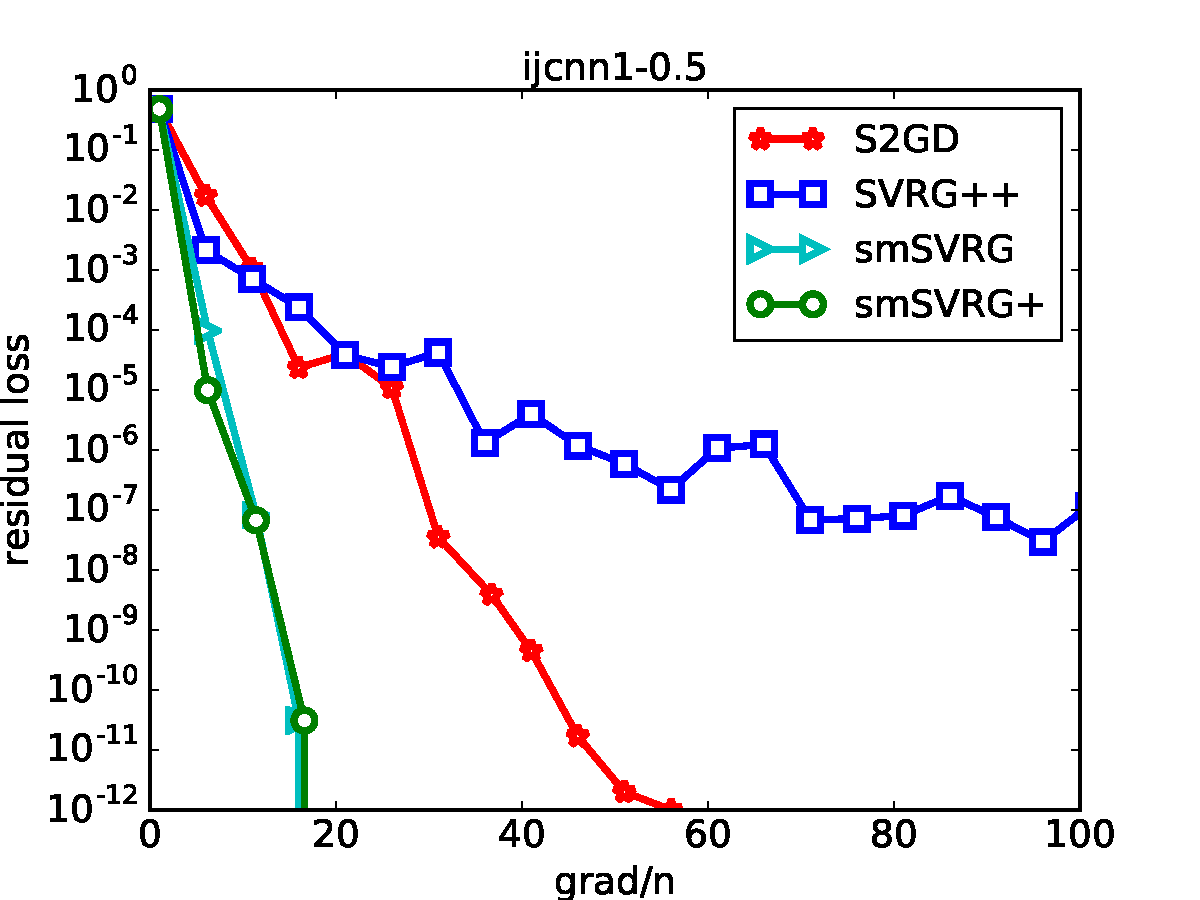
\includegraphics[width=0.24\linewidth]{cmijcnn105}\label{cmijcnn105}}
\subfigure[ijcnn1 $\eta=0.05$]{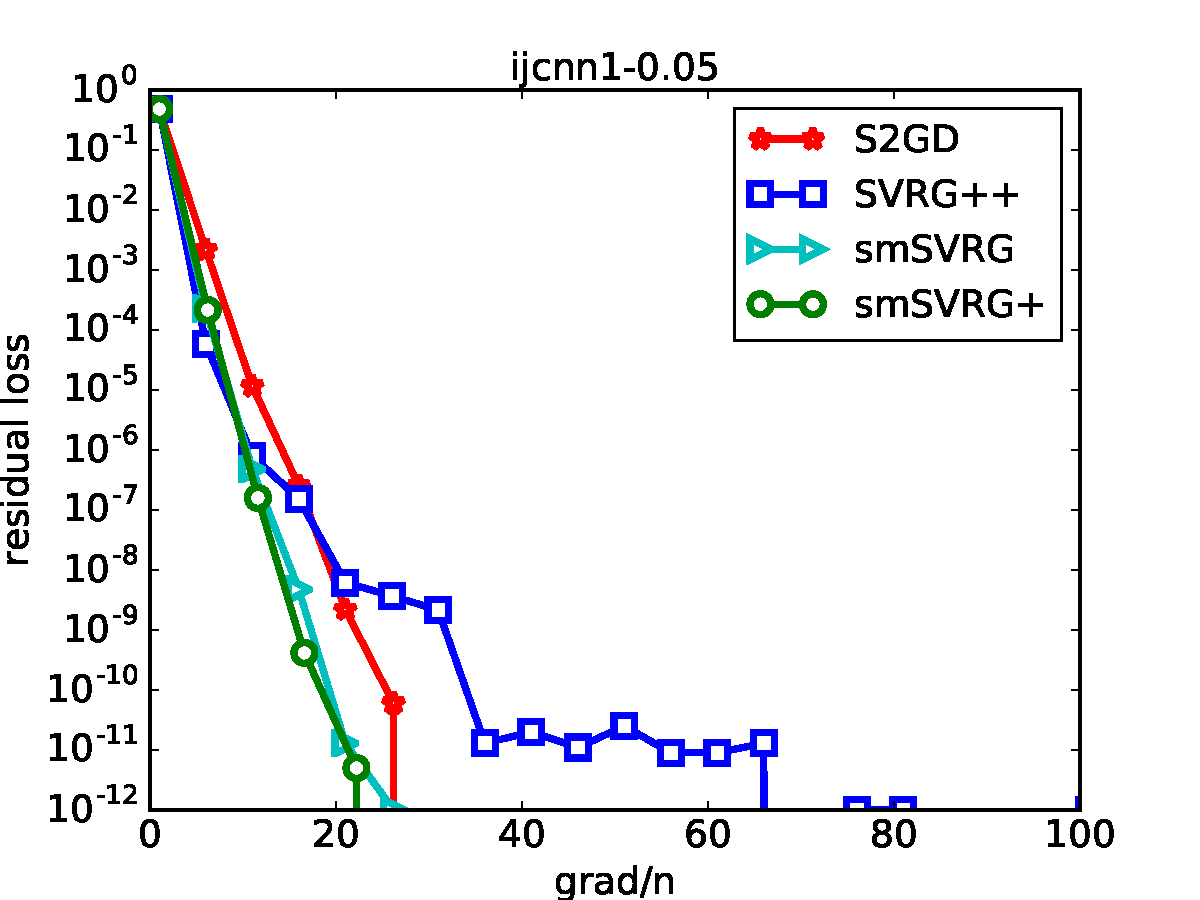
\includegraphics[width=0.24\linewidth]{cmijcnn1005}\label{cmijcnn1005}}
\subfigure[ijcnn1 $\eta=0.01$]{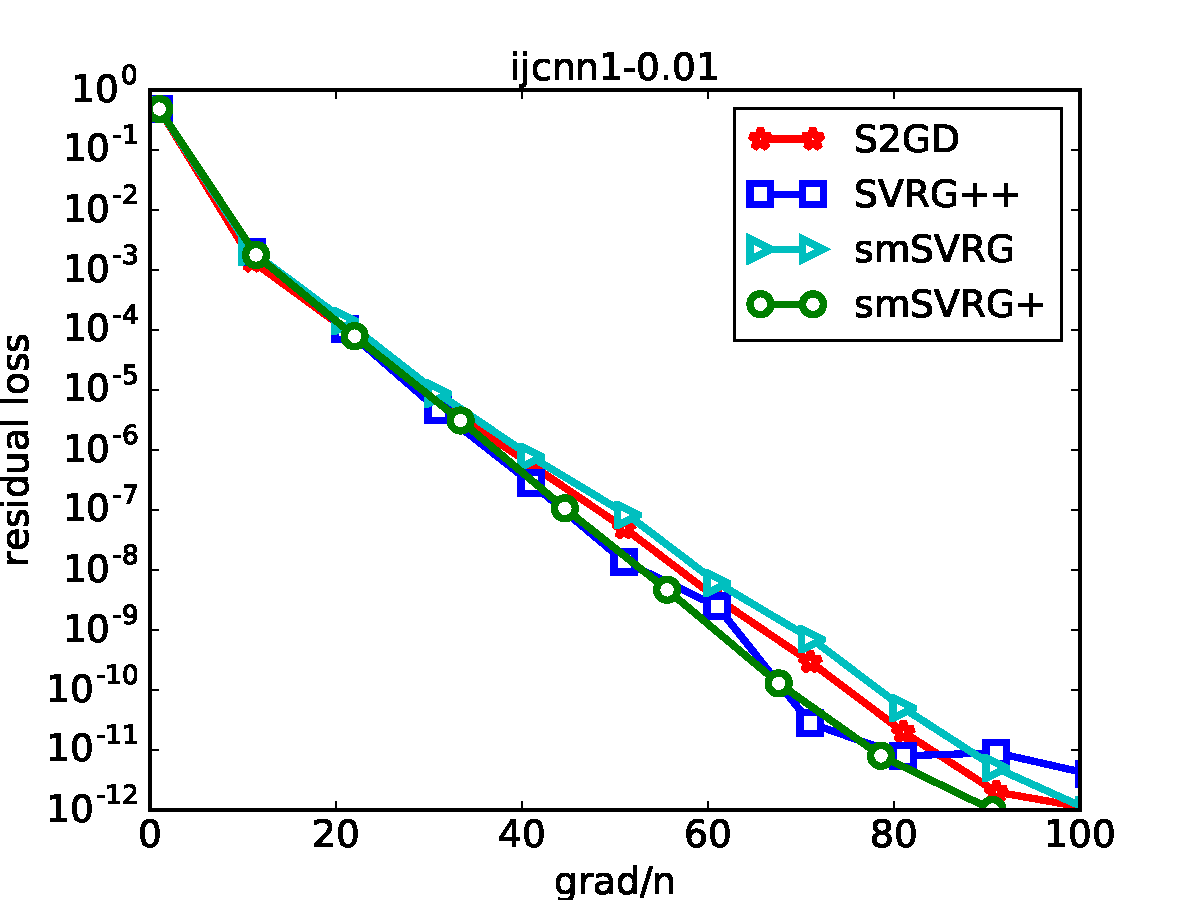
\includegraphics[width=0.24\linewidth]{cmijcnn1001}\label{cmijcnn1001}}
\subfigure[ijcnn1 $\eta=0.001$]{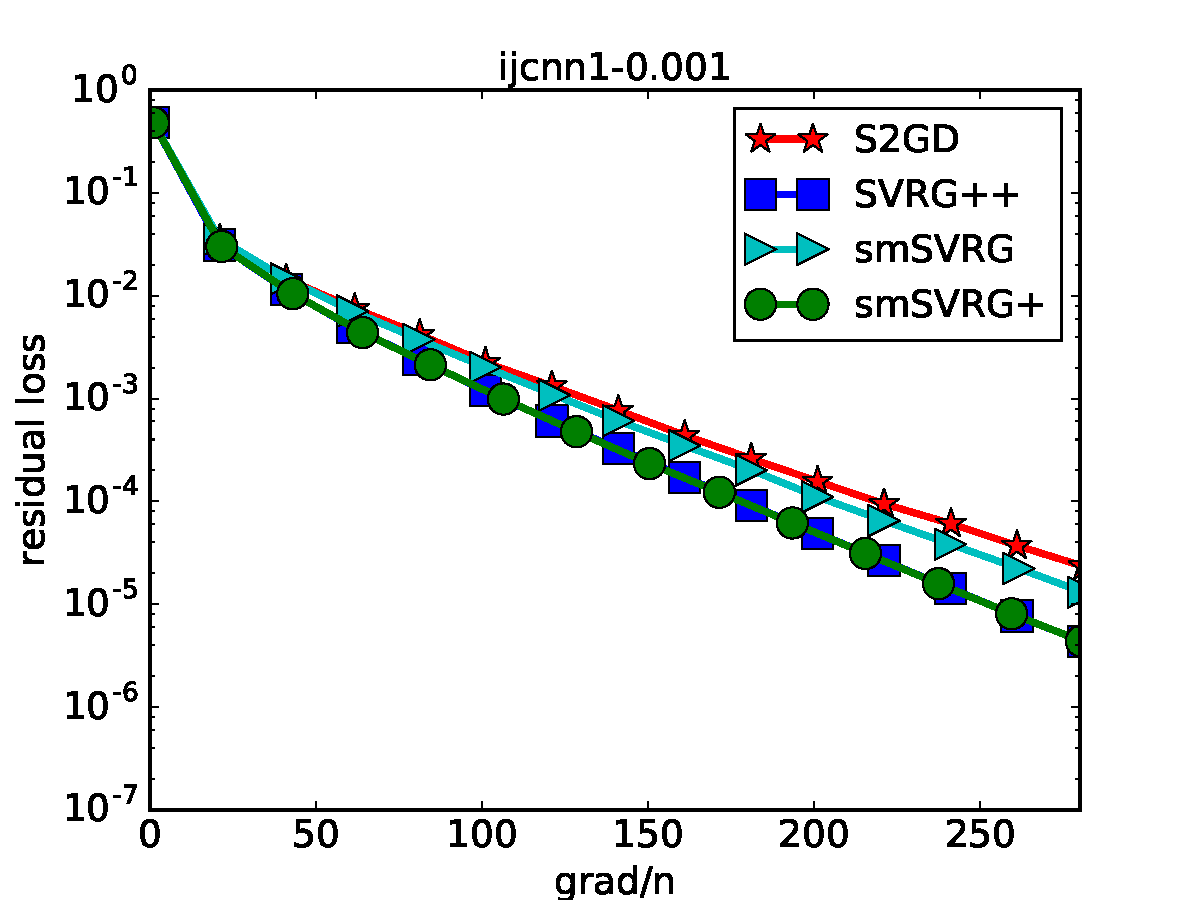
\includegraphics[width=0.24\linewidth]{cmijcnn10001}\label{cmijcnn10001}}
\label{cmijcnn1}
\caption{Comparison of \textsc{smSVRG}, \textsc{smSVRG+}, SVRG++, S2GD}
\end{figure*}
 
 \section{Numerical Experiments}
 \label{numexperiments}
 %\subsection{Experimental settings}
 In this section, we conduct some experiments to demonstrate the efficiency of our proposed algorithm. We evaluate our algorithm on four training datasets, which are public on the LIBSVM website\footnote{http://www.csie.ntu.edu.tw/$\sim$cjlin/libsvmtools/datasets/}. In our experiments, \textsc{smSVRG} is applied for two standard machine learning tasks: $l2$-regularized logistic regression and $l2$-regularized ridge regression.
 
 The $l2$-regularized logistic regression task is conducted on the two datasets: ijcnn1, a9a. Since the label of each instance in these datasets is set to be 1 or -1, the loss function of $l2$-regularized logistic regression task is:
\begin{equation}
\label{logistic_reg}
\min\limits_\omega \frac{1}{n}\sum\limits_{i=1}^n \log(1+e^{-y_i \omega^\mathrm{T} x_i }) + \lambda \parallel \omega \parallel^2.
\end{equation}
The $l2$-regularized ridge regression task is conducted on the four datasets: YearPredictMSD, and cadata. The loss function of $l2$-regularized ridge regression task is:
\begin{equation}
\label{ridge_reg}
\min\limits_\omega \frac{1}{n}\sum\limits_{i=1}^n\left(\omega^{\mathrm{T}}x_i-y_i\right)^2 + \lambda \parallel \omega \parallel^2.
\end{equation}
We scale the value of all features to $[-1,1]$ and set the weighting parameter $\lambda$ to $10^{-4}$ for all evaluations. 
In all figures, the $x$-axis denotes the computational cost, which is measured by the number of gradient computation divided by the size of training data, i.e. $n$. The $y$-axis denotes training loss residual, i.e. $F(\tilde{\omega}_s) - F(\omega^{*})$. Note that the optimum $\omega^*$ is estimated by running the gradient descent for a long time. Our numerical experiments include two parts: comparing with existing related methods and comparing with SVRG of different epoch sizes. Both experiments show the superior performance of our methods. 

\begin{table}[]
\centering
\caption{Detail information of datasets and models}
\label{data information}
\begin{tabular}{|l|l|l|l|l|}
\hline
Dataset           & size & dimension & model & $\lambda$ \\ \hline
ijcnn1            &  49990 &  22 &   logistic    &  $10^{-4}$         \\
a9a               &   32561&123   &     logistic  &      $10^{-4}$     \\ 
YearPredictionMSD & 463715  &  90 &    linear  &      $10^{-4}$     \\
cadata              & 20640  &8   &     linear  &    $10^{-4}$       \\ \hline
\end{tabular}
\end{table}



\subsection{Comparing with existing related methods}
In this section, we compare our \textsc{smSVRG} and \textsc{smSVRG+} with two aforementioned existing methods: SVRG++ and S2GD. We do not compare with SVRG\_Auto\_Epoch in that we find its termination condition of epoch is never satisfied and keeps doing SGD iteration, resulting in nonconvegence. For SVRG++, we initialize $m = n$. For S2GD, we set the maximum of $m$ to be $4n$. For both \textsc{smSVRG} and \textsc{smSVRG+}, we set the window size, i.e. $m_0$ to be $n/10$.We evaluate these methods by running logistic regression on dataset ijcnn1. 
As illustrated in Figure \ref{figure_logistic_ijcnn}, we can see that SVRG++ fluctuates violently and fails to converge due to the large variance caused by too large epoch size. It only performs well when $\eta$ is quite small. As shown in Figures \ref{cmijcnn105}, \ref{cmijcnn1005}, both \textsc{smSVRG} and \textsc{smSVRG+} converge rapidly with the relatively large $\eta$ because  they can constrain $m$ in a small range. However, it can be seen from Figures \ref{cmijcnn1001}, \ref{cmijcnn10001}, when $\eta$ decreases to a small value, the performance of \textsc{smSVRG} drops gradually and even becomes inferior to others, while \textsc{smSVRG+} always performs better than its countparts. The main reason is that  when $\eta$ is small, more iterations can be computed in one epoch, thus checking the inequality frequently will resulting algorithm to stop epochs too early. The strategy of increase of window size applied by \textsc{smSVRG+} can reduce the variance. Hence it always outperforms other methods.



\begin{figure*}[ht]
\centering
\subfigure[ijcnn1 $\eta=0.5$]{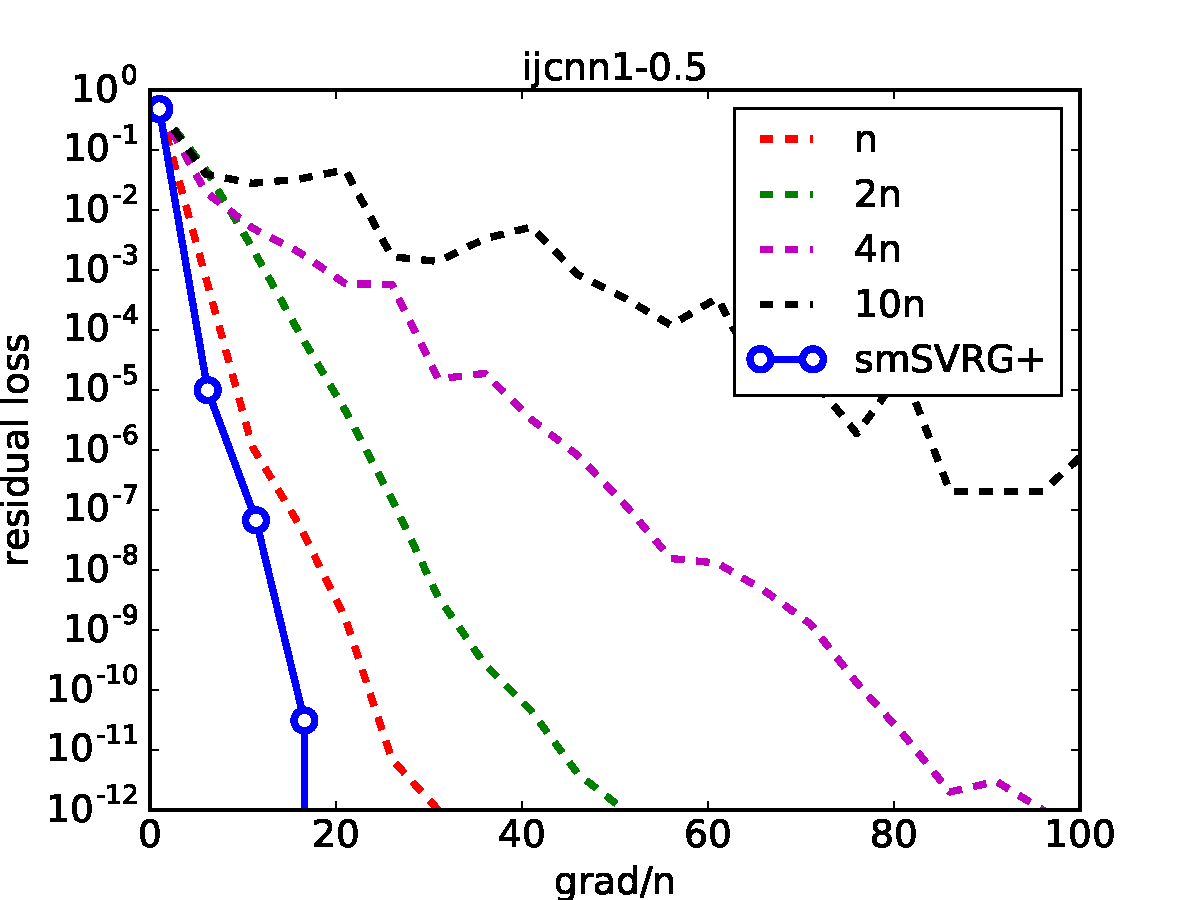
\includegraphics[width=0.5\columnwidth]{ijcnn105}\label{ijcnn105}}
\subfigure[ijcnn1 $\eta=0.05$]{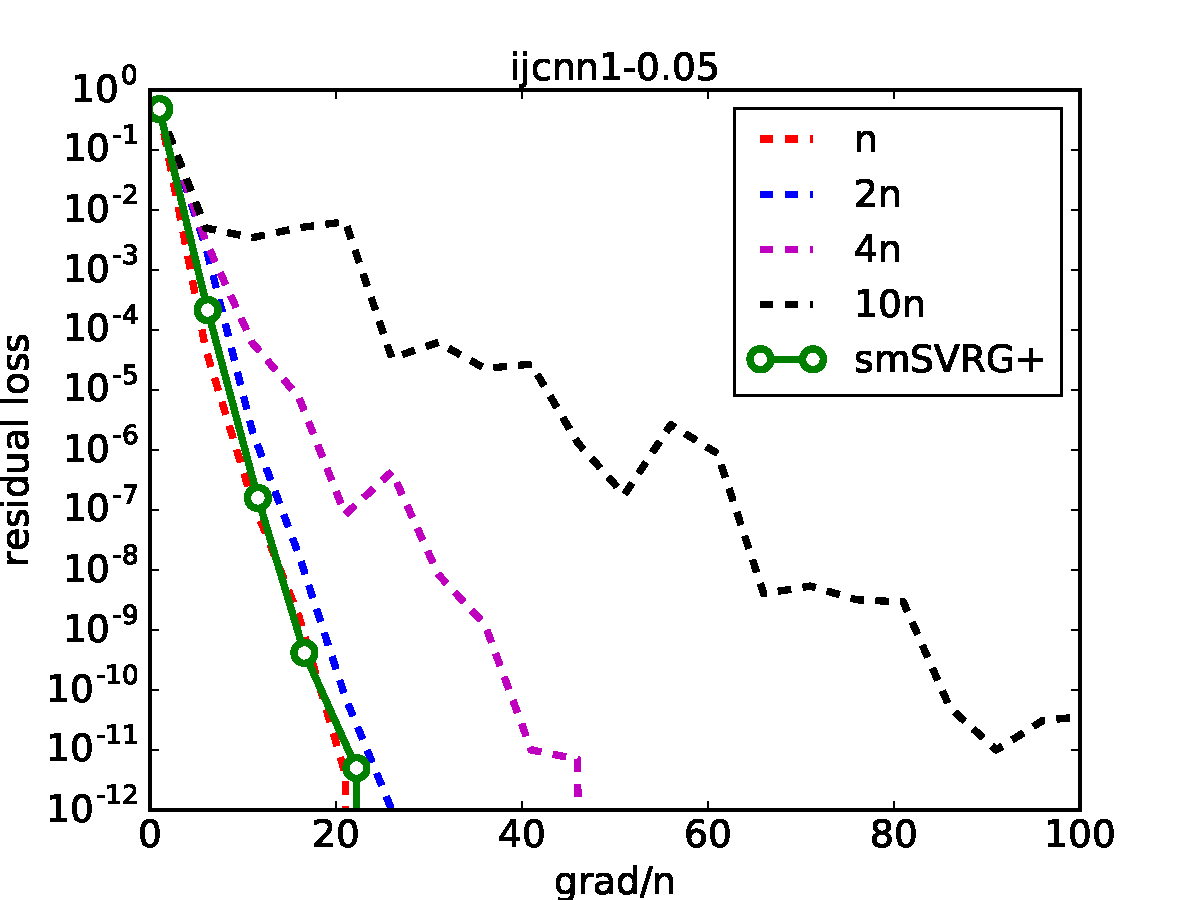
\includegraphics[width=0.5\columnwidth]{ijcnn1005}\label{ijcnn1005}}
\subfigure[ijcnn1 $\eta=0.01$]{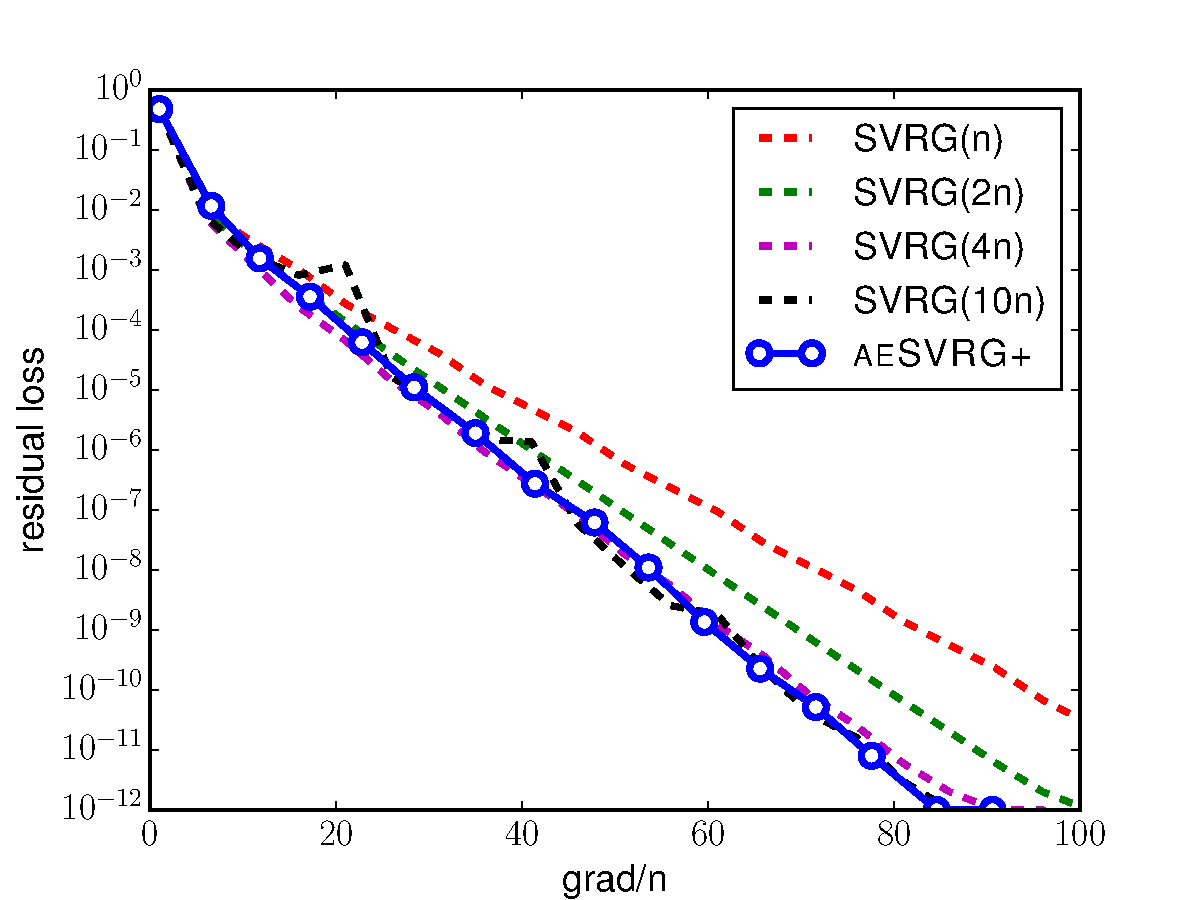
\includegraphics[width=0.5\columnwidth]{ijcnn1001}\label{ijcnn1001}}
\subfigure[ijcnn1 $\eta=0.001$]{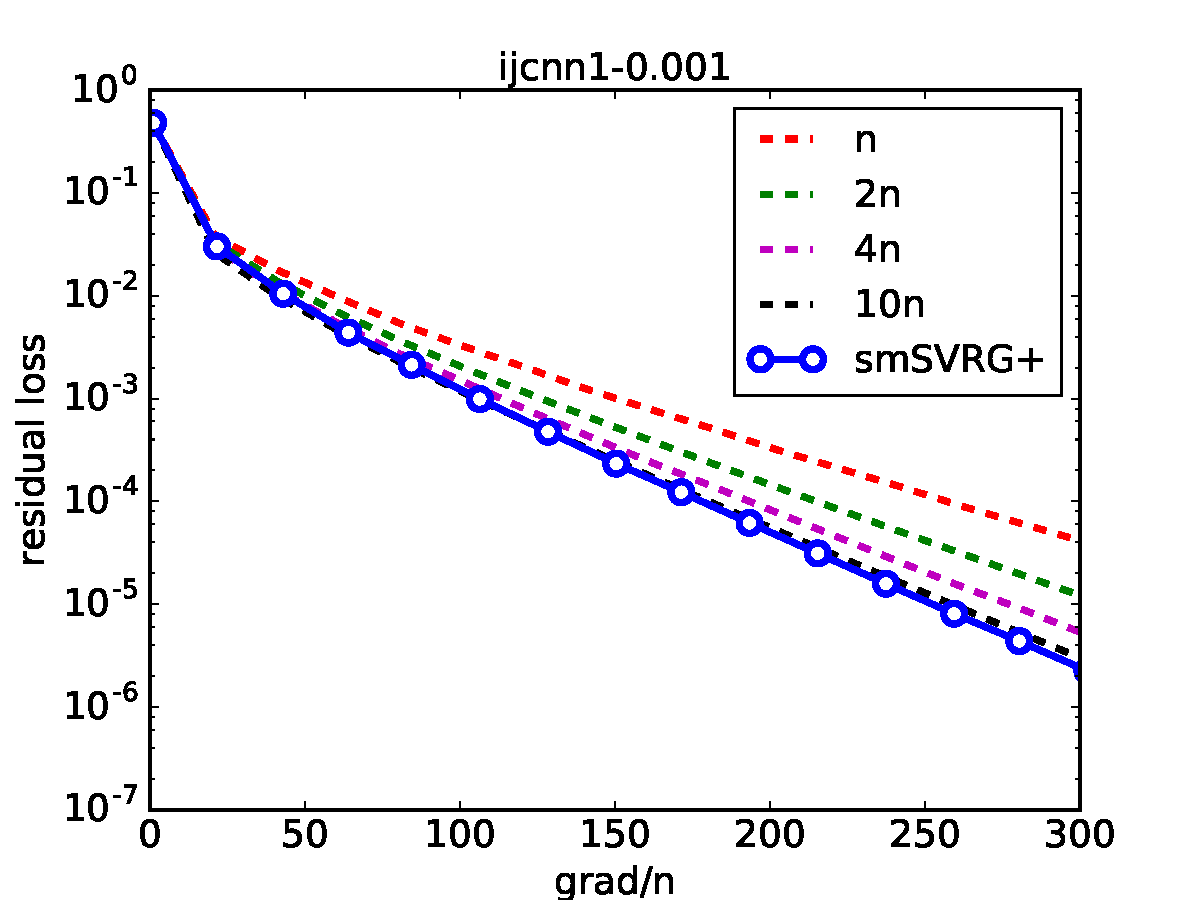
\includegraphics[width=0.5\columnwidth]{ijcnn10001}\label{ijcnn10001}}
\label{figure_logistic_ijcnn}
\caption{Generally, \textsc{smSVRG} can automatically set an appropriate $m$ with different learning rates for the $l2$-regularized logistic regression}
\end{figure*}

\begin{figure*}[ht]
\centering
\subfigure[a9a $\eta=0.3$]{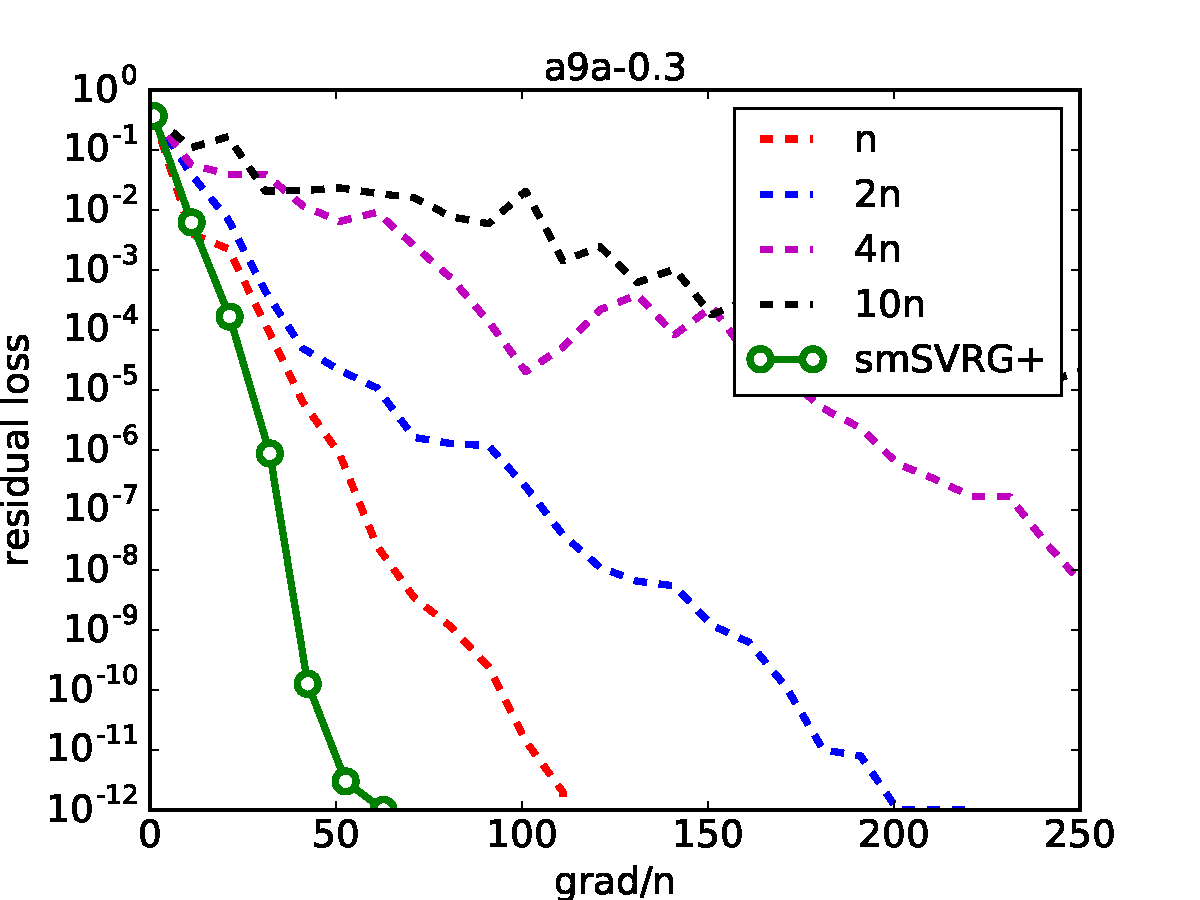
\includegraphics[width=0.5\columnwidth]{a9a03}\label{a9a03}}
\subfigure[a9a $\eta=0.05$]{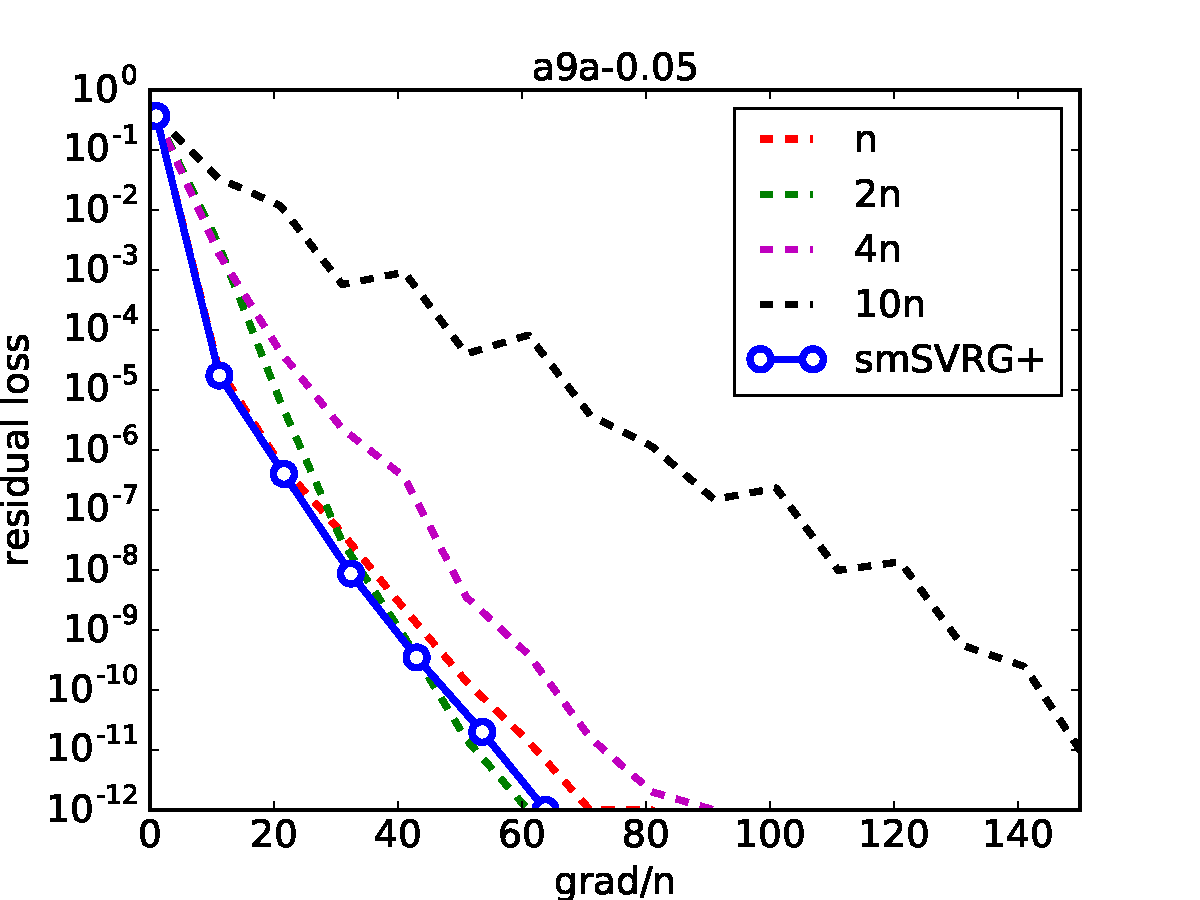
\includegraphics[width=0.5\columnwidth]{a9a005}\label{a9a005}}
\subfigure[a9a $\eta=0.02$]{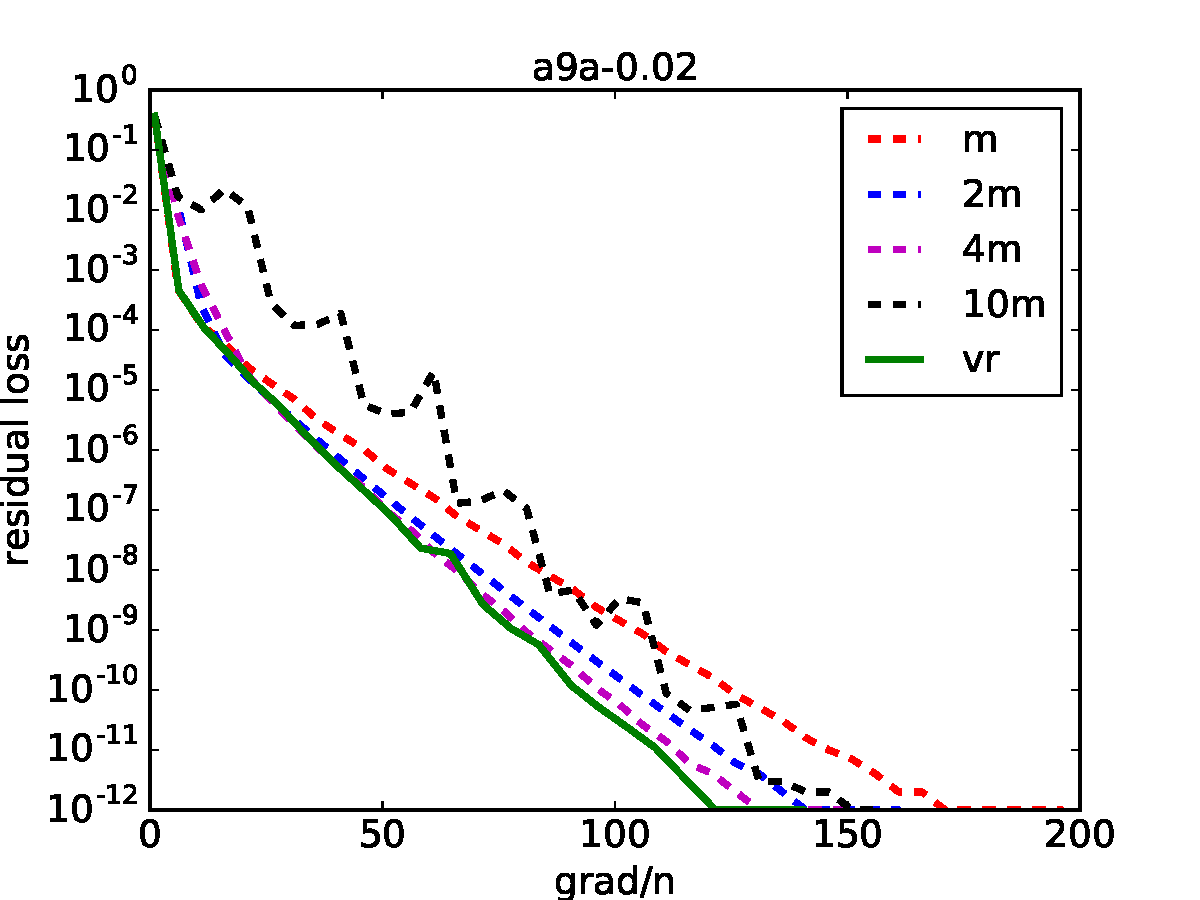
\includegraphics[width=0.5\columnwidth]{a9a002}\label{a9a002}}
\subfigure[a9a $\eta=0.001$]{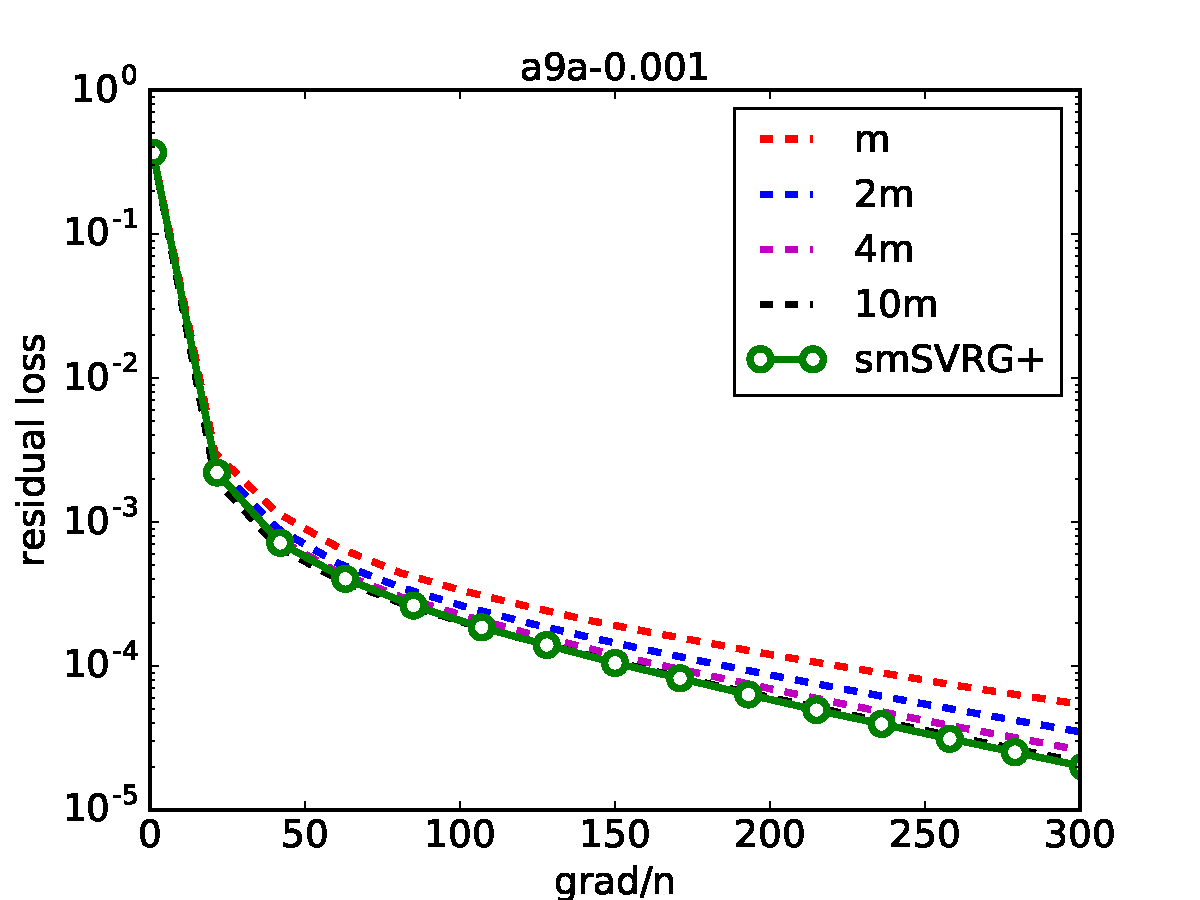
\includegraphics[width=0.5\columnwidth]{a9a0001}\label{a9a0001}}
\label{figure_logistic_a9a}
\caption{Generally, \textsc{smSVRG} can automatically set an appropriate $m$ with different learning rates for the $l2$-regularized logistic regression}
\end{figure*}



\begin{figure*}[t]
\subfigure[YearPredictionMSD $\eta=0.01$]{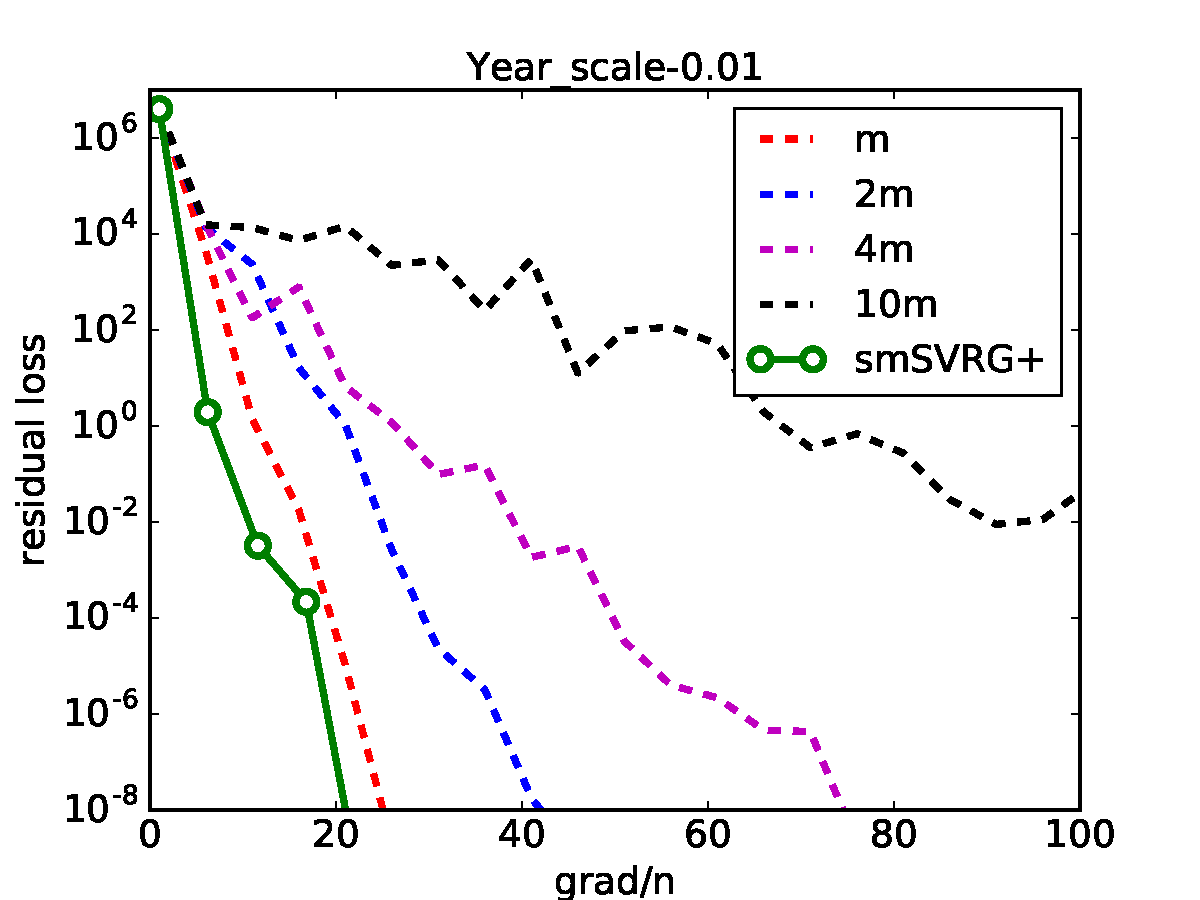
\includegraphics[width=0.5\columnwidth]{Year_scale001}\label{Year_scale001}}
\subfigure[YearPredictionMSD $\eta=0.005$]{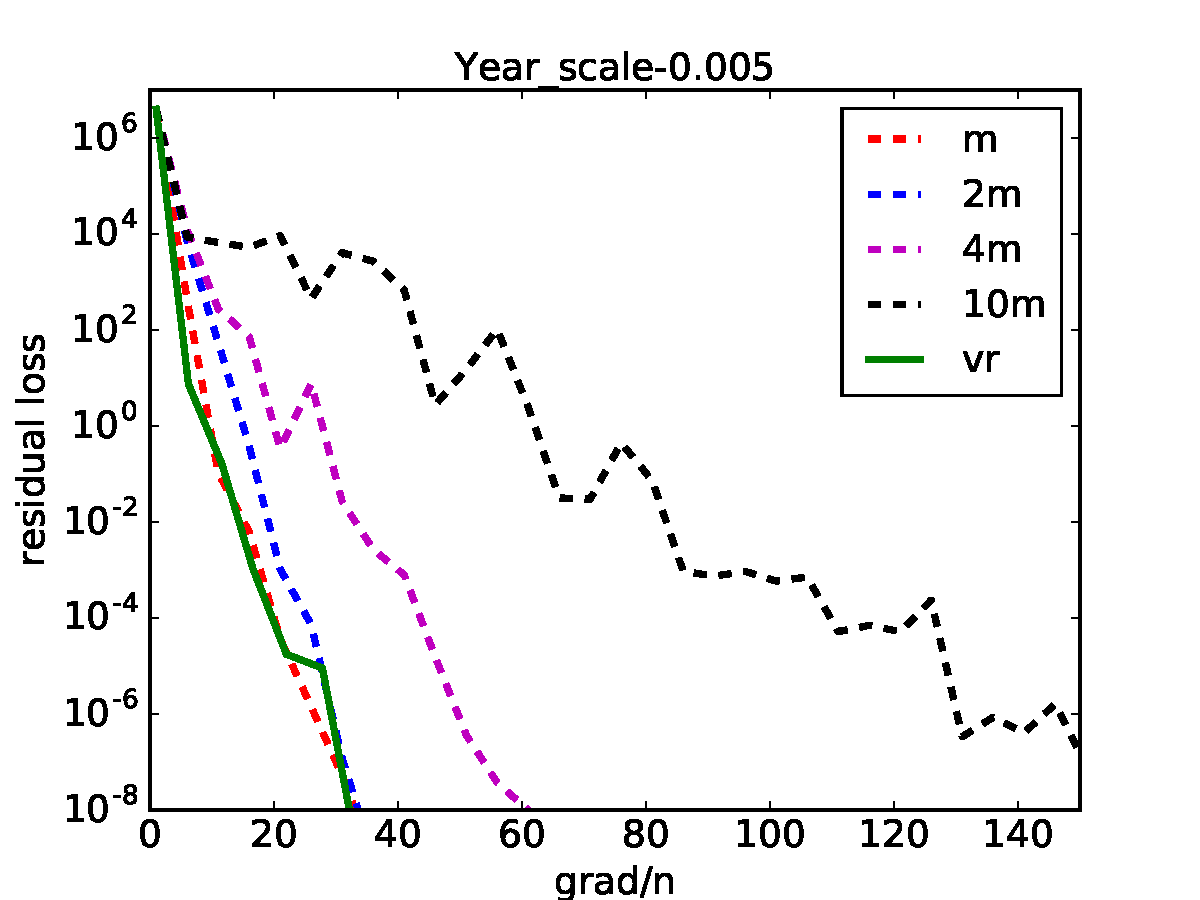
\includegraphics[width=0.5\columnwidth]{Year_scale0005}\label{Year_scale0005}}
\subfigure[YearPredictionMSD $\eta=0.002$]{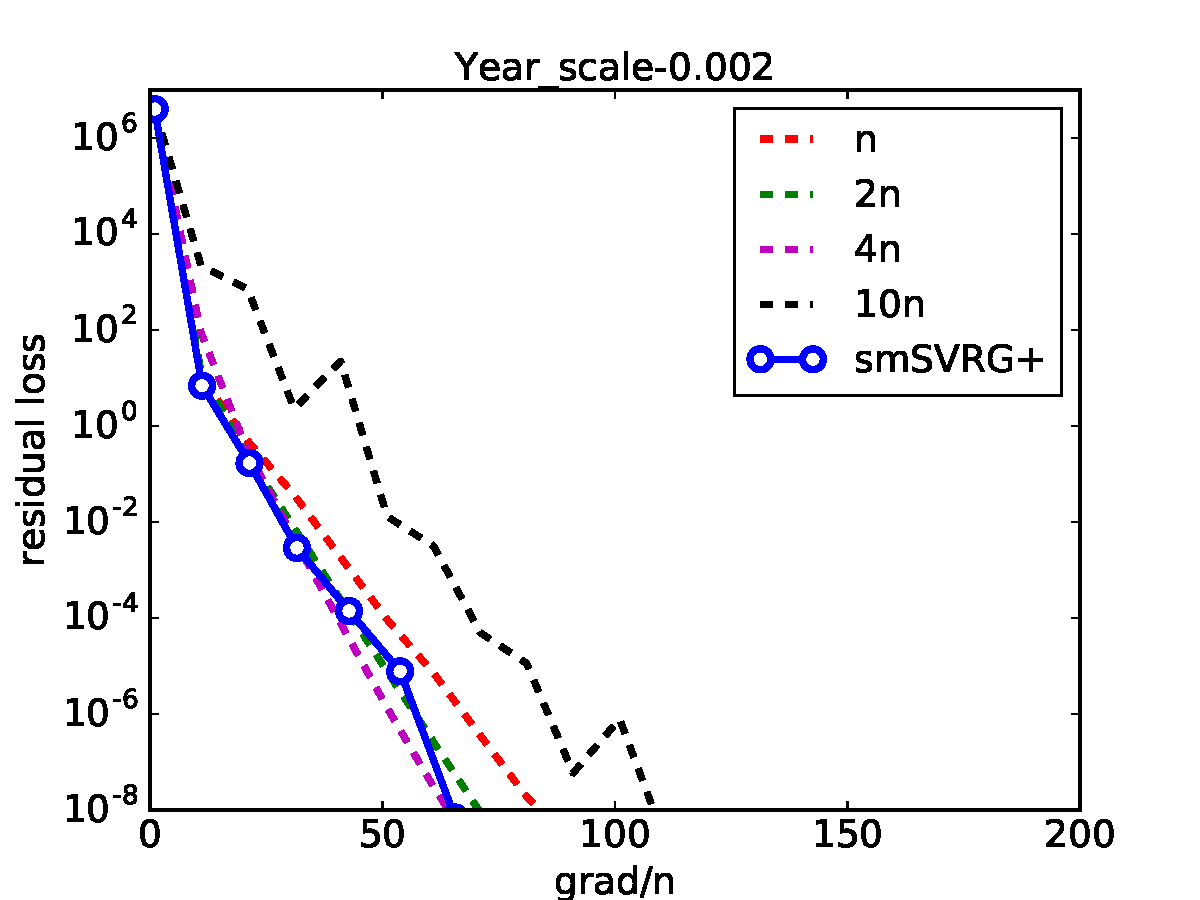
\includegraphics[width=0.5\columnwidth]{Year_scale0002}\label{Year_scale0002}}
\subfigure[YearPredictionMSD $\eta=0.0001$]{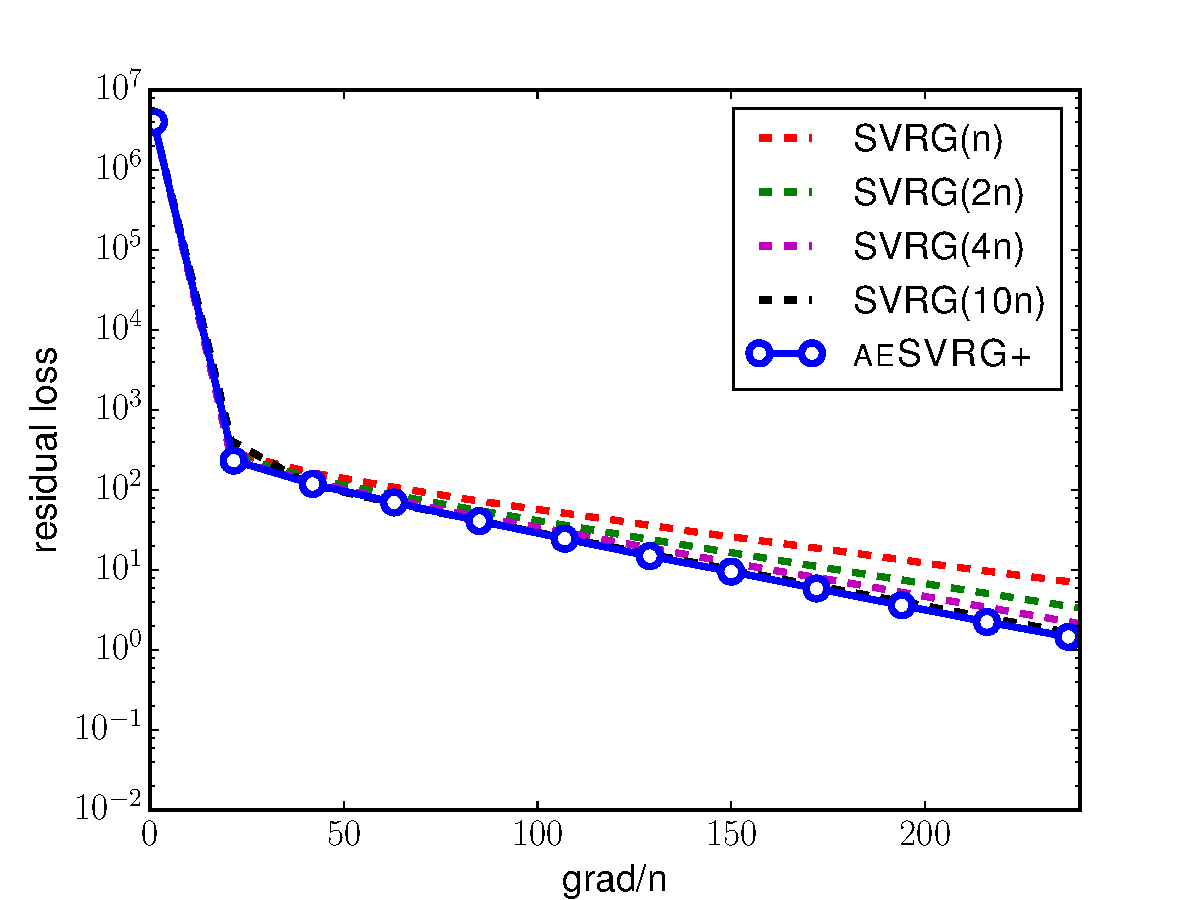
\includegraphics[width=0.5\columnwidth]{Year_scale00001}\label{Year_scale00001}}
\label{figure_linear_scale}
\caption{Generally, \textsc{smSVRG} can automatically set an appropriate $m$ with different learning rates for the $l2$-regularized linear regression}
\end{figure*}

\begin{figure*}[t]
\subfigure[cadata $\eta=0.1$]{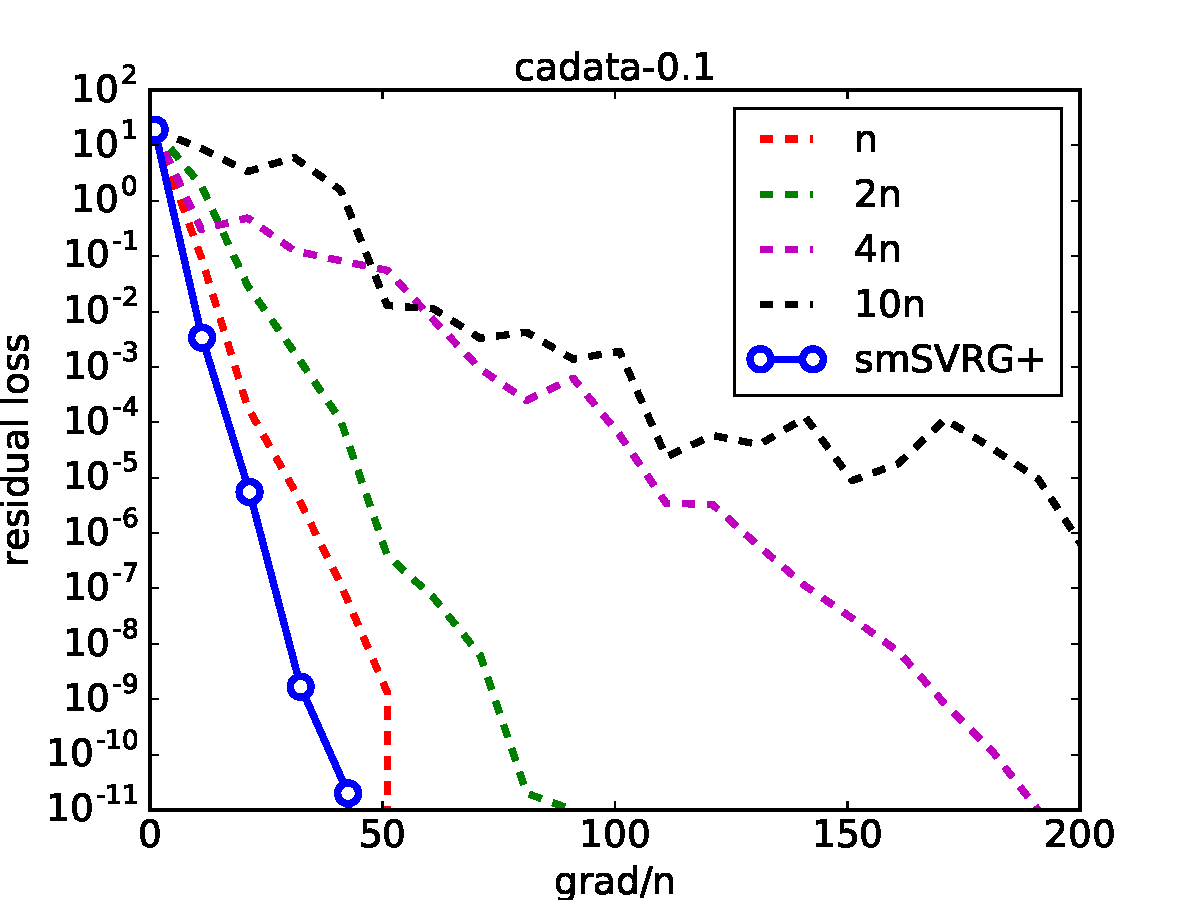
\includegraphics[width=0.5\columnwidth]{cadata01}\label{cadata01}}
\subfigure[cadata $\eta=0.05$]{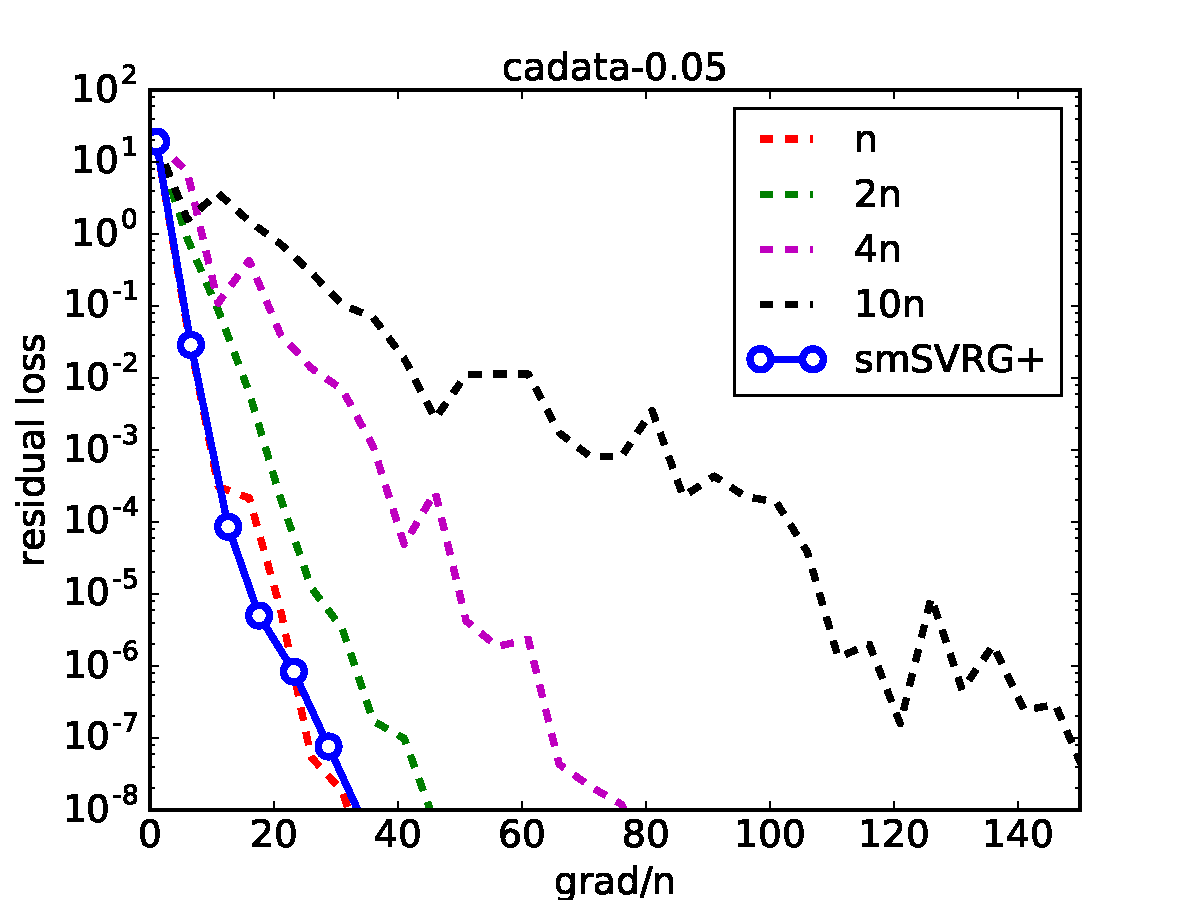
\includegraphics[width=0.5\columnwidth]{cadata005}\label{cadata005}}
\subfigure[cadata $\eta=0.02$]{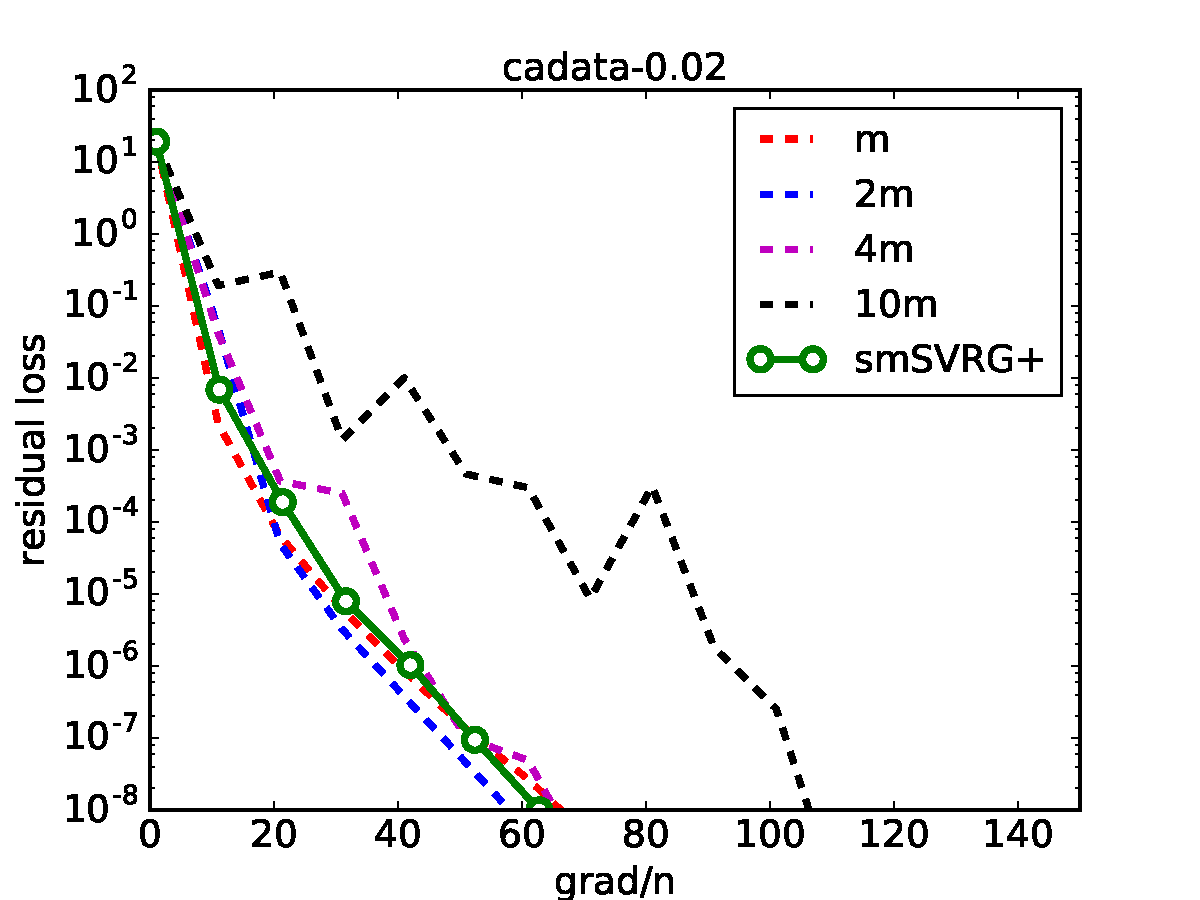
\includegraphics[width=0.5\columnwidth]{cadata002}\label{cadata002}}
\subfigure[cadata $\eta=0.001$]{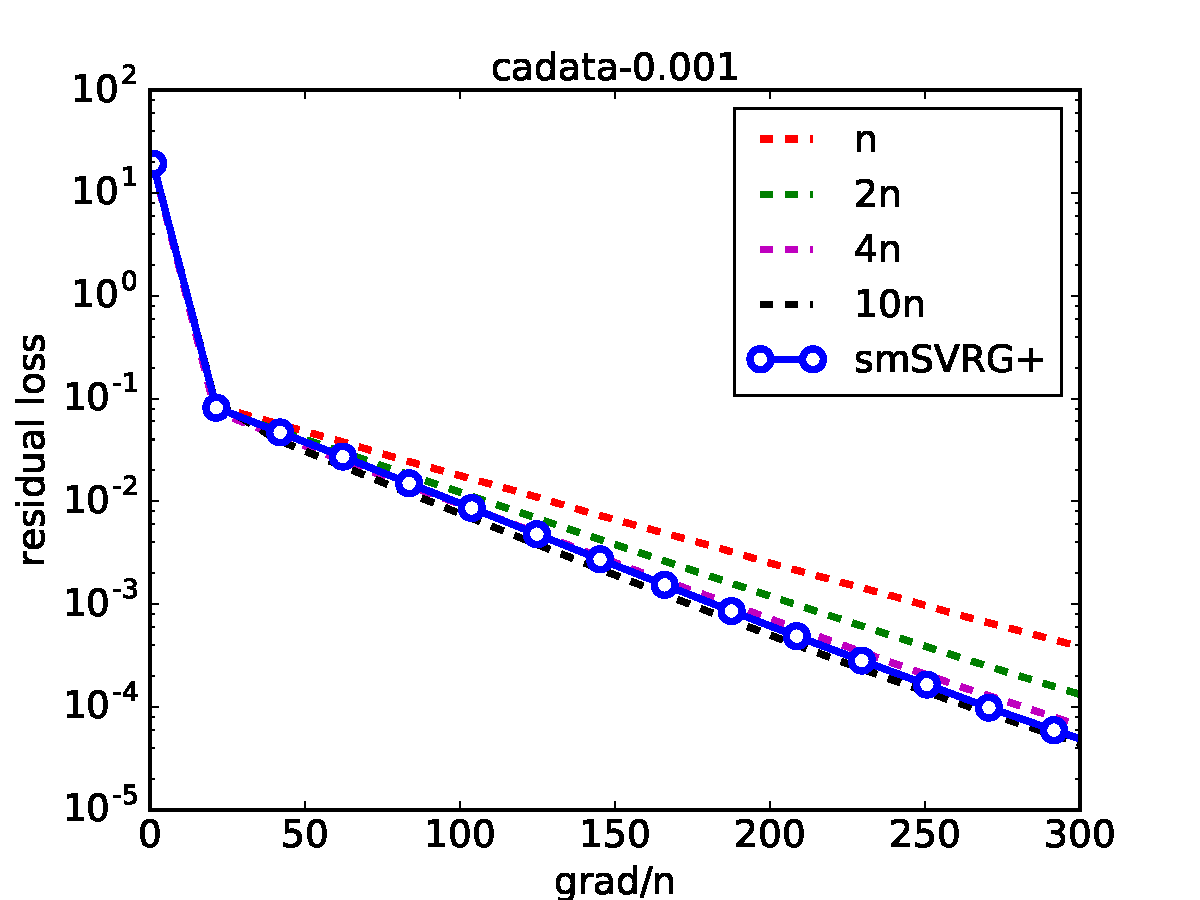
\includegraphics[width=0.5\columnwidth]{cadata0001}\label{cadata0001}}
\label{figure_linear_cadata}
\caption{Generally, \textsc{smSVRG} can automatically set an appropriate $m$ with different learning rates for the $l2$-regularized linear regression}
\end{figure*}


 \subsection{Comparing with SVRG by varying learning rate}
Since \textsc{smSVRG+} performs better than \textsc{smSVRG}, \textsc{smSVRG+} is used to conduct the comparison with SVRG. For SVRG, we increase the epoch size, i.e. $m$ as four different values: $n$, $2n$, $4n$, $10n$. The first three values are chosen for the reason that they are commonly used in most previous researches \citep{aaa, bbb}. Besides, our experiments show that epoch size which is large than $10n$ leads to much variance and slows the convergence of the training loss. It is easy to comprehend that the full gradient computation becomes less important when epoch size is rather large. In other words, SVRG with an extremely large epoch size degenerates to SGD. In all figures, the dashed lines represents SVRG with fixed epoch size; while the green solid lines stands for \textsc{smSVRG+}.
 
As illustrated in Figures \ref{figure_linear_scale} and \ref{figure_linear_cadata},  \textsc{smSVRG+} can always have the similar performance as SVRG with most best-tuned epoch size. We observe that when $\eta$ is large,  and $m$ is set to be a small value, e.g. $n$, can achieve best performance. The main reason is that when $\eta$ is large, the variance becomes significant simultaneously, so $m$ must be set to be small in order to bound the variance. As $\eta$ decays, the optimal value of $m$ increases, which means that the algorithm can tolerate more variance induced by extra iterations. As illustrated in Figures \ref{aaaa, bbbb}, our method is comparable to and sometimes even better than SVRG with best-tuned epoch sizes when learning rate is large or medium. However, if $\eta$ is set to be too small, \textsc{smSVRG+} performs slightly inferior to  SVRG with large epoch sizes, but outperforms SVRG with recommended epoch sizes, i.e. $n$ and $2n$. It is noting that setting $\eta$ to be too small is not a practical approach when using SVRG or its variants, because the convergence rate will be extremely low. Therefore, the sub-optimal performance of \textsc{smSVRG+} with very small $\eta$ is acceptable.
 

 

\section{Conclusion}
\label{conclusion}
1111

111

111

111

111




% trigger a \newpage just before the given reference
% number - used to balance the columns on the last page
% adjust value as needed - may need to be readjusted if
% the document is modified later
%\IEEEtriggeratref{8}
% The "triggered" command can be changed if desired:
%\IEEEtriggercmd{\enlargethispage{-5in}}

% references section

% can use a bibliography generated by BibTeX as a .bbl file
% BibTeX documentation can be easily obtained at:
% http://mirror.ctan.org/biblio/bibtex/contrib/doc/
% The IEEEtran BibTeX style support page is at:
% http://www.michaelshell.org/tex/ieeetran/bibtex/
%\bibliographystyle{IEEEtran}
% argument is your BibTeX string definitions and bibliography database(s)
%\bibliography{IEEEabrv,../bib/paper}
%
% <OR> manually copy in the resultant .bbl file
% set second argument of \begin to the number of references
% (used to reserve space for the reference number labels box)


%\begin{thebibliography}{1}
%\bibitem{IEEEhowto:kopka}
%H.~Kopka and P.~W. Daly, \emph{A Guide to \LaTeX}, 3rd~ed.\hskip 1em plus
 % 0.5em minus 0.4em\relax Harlow, England: Addison-Wesley, 1999.
%\end{thebibliography}
%\newpage
\newpage
\bibliographystyle{plain}
\bibliography{reference}


% that's all folks
\end{document}


